% !TeX root = ../../Book1.tex
% 纲要标题：### 8.2 法向几何与第二基本形式
% 纲要位置：几何学计划纲要.md，第 409 行。
% 正文状态：初稿；尚未正式审核。

% 纲要内容开始
% 
% * Gauss 映射和形算子
% * 主曲率、法曲率与 Euler 公式
% * 平均曲率、Gauss 曲率及脐点
% * 曲率线、渐近线及其退化
% 
% 纲要内容结束

\section{法向几何与第二基本形式}
\label{g1:sec:0802}

一张纸卷成圆柱后，小范围内的长度和角度没有改变，切平面却随着位置转动。第一基本形式记录前一种信息；要描述后一种变化，就应比较邻近点的法向量。曲线只有一个切方向，曲面在一点有整整一圈方向，因此需要一个线性算子同时记录沿各方向前进时法向量怎样变化。以下所有曲面参数均为光滑浸入 \(X:U\to\mathbb R^3\)，其中 \(U\subset\mathbb R^2\) 为开集；讨论在参数邻域中进行，自交处的不同分支分别处理。

\subsection{Gauss 映射和形算子}
\label{g1:subsec:0802:01}

令 \(X_i=\partial X/\partial u^i\)。上一节的正则性保证 \(X_1\times X_2\ne0\)，因而在每张参数片上可以选择光滑单位法向
\[
	n=\frac{X_1\times X_2}{\sqrt D},\qquad
	D=EG-F^2,\quad E=\langle X_1,X_1\rangle,\quad F=\langle X_1,X_2\rangle,\quad G=\langle X_2,X_2\rangle.
\]
也可以选相反的 \(n\)。以下先固定这一选择；曲面若不能作整体的法向选择，这些构造仍可在每张小参数片上使用。

\begin{definition}[Gauss 映射与形算子]\label{g1:def:shape-operator}
	设 \(X:U\to\mathbb R^3\) 为光滑浸入，\(n:U\to S^2\) 为一个光滑单位法向场。把每一点送到其单位法向的映射 \(n\) 称为\term[Gaussyingshe]{Gauss 映射}[Gauss map]。\footnote{Gauss（高斯，Carl Friedrich Gauss，1777--1855）是德国数学家，在数论、微分几何与测地学等领域作出重要贡献。}对每个参数点 \(q\in U\)，令 \(p=X(q)\)，并在这一参数分支上定义\term[xingsuanzi]{形算子}[shape operator]
	\[
		S_q:\mathrm{T}_qX\longrightarrow \mathrm{T}_qX,\qquad
		S_q\!\left(\sum_i a^iX_i\right)=-\sum_i a^i n_i.
	\]
	它也记为 \(S=-\mathrm dn\)，其中用 \(\mathrm dX\) 把参数切向量与曲面切向量对应起来。
	\symidx{\(S\)：曲面的形算子 \(S=-\mathrm dn\)}
\end{definition}

这个定义中有两个需要核对的地方。首先，\(X_1,X_2\) 线性无关，所以系数 \(a^i\) 唯一；其次，对 \(\langle n,n\rangle=1\) 求导得到 \(\langle n_i,n\rangle=0\)，故 \(n_i\) 确实落在 \(\mathrm{T}_qX=n^\perp\) 中。Gauss 映射的微分本来取值于 \(\mathrm{T}_{n(q)}S^2\)，这里使用了这两个切平面作为 \(\mathbb R^3\) 线性子空间恰好都是 \(n^\perp\) 的事实。

\ProseParagraphBreak

负号使“曲线的法向加速度”稍后直接等于形算子的二次型。它也决定了球面的符号：半径 \(R\) 的球面若取外向法向 \(n(q)=p/R\)，则 \(\mathrm dn(v)=v/R\)，所以 \(S=-I/R\)。不要把别处采用 \(S=\mathrm dn\) 的主曲率公式直接移入这里。

\begin{definition}[第二基本形式]\label{g1:def:second-fundamental-form}
	在带选定单位法向的光滑浸入曲面上，对每个参数点 \(q\) 定义
	\[
		\mathrm{II}_q(v,w)\coloneqq\langle S_qv,w\rangle,\qquad v,w\in \mathrm{T}_qX.
	\]
	这个双线性型称为\term[dierjibenxingshi]{第二基本形式}[second fundamental form]。它的对称性由下面的计算给出。在坐标中记 \(h_{ij}=\mathrm{II}(X_i,X_j)\)，于是
	\[
		\mathrm{II}=h_{11}(\mathrm du^1)^2+2h_{12}\,\mathrm du^1\mathrm du^2+h_{22}(\mathrm du^2)^2.
	\]
	\symidx{\(\mathrm{II}\)：第二基本形式}
	\symidx{\(h_{ij}\)：第二基本形式的坐标系数}
\end{definition}

\begin{proposition}[形算子的自伴性与坐标表示]\label{g1:prop:shape-self-adjoint}
	设 \(X:U\to\mathbb R^3\) 为光滑浸入，并选定光滑单位法向 \(n\)。则
	\begin{equation}\label{g1:eq:second-form-coefficients}
		h_{ij}=-\langle n_i,X_j\rangle=\langle X_{ij},n\rangle.
	\end{equation}
	第二基本形式对称，形算子关于第一基本形式自伴，即 \(\langle Sv,w\rangle=\langle v,Sw\rangle\)。以列向量表示系数时，形算子在基 \(X_1,X_2\) 下的矩阵为
	\begin{equation}\label{g1:eq:shape-matrix}
		[S]=g^{-1}h,\qquad g=(g_{ij}),\quad h=(h_{ij}).
	\end{equation}
	若作光滑坐标变换 \(u=u(v)\)，令 \(A=(\partial u^i/\partial v^a)\)，并保留同一个几何法向场，则 \(\widetilde h=A^{\mathsf T}hA\)。因此 \(\mathrm{II}\) 不依赖参数的选择。
\end{proposition}
\begin{proof}
	对 \(\langle n,X_j\rangle=0\) 关于 \(u^i\) 求导，得到 \(\langle n_i,X_j\rangle+\langle n,X_{ij}\rangle=0\)。混合偏导相等给出 \(h_{ij}=h_{ji}\)，再由双线性性得到自伴性。若 \(S(X_j)=\sum_i S^i{}_jX_i\)，则
	\[
		\sum_i g_{ki}S^i{}_j=\langle X_k,S(X_j)\rangle=h_{kj}.
	\]
	即 \(g[S]=h\)，而 \(g\) 正定可逆，故得\eqref{g1:eq:shape-matrix}。

	对 \(\widetilde X(v)=X(u(v))\) 两次求导，有
	\[
		\widetilde X_{ab}=\sum_{i,j}X_{ij}A^i{}_aA^j{}_b+\sum_i X_i\frac{\partial^2u^i}{\partial v^a\partial v^b}.
	\]
	与 \(n\) 作内积后，第二项消失，第一项正是 \((A^{\mathsf T}hA)_{ab}\)。变换后的切向量系数代入这个式子，双线性型的值保持不变。
\end{proof}

这里的自伴性由内积 \(g\) 衡量。一般参数的 \(X_1,X_2\) 不一定正交，矩阵 \(g^{-1}h\) 因而未必等于自己的转置；直接把它当作标准内积下的对称矩阵，会混淆两个不同的内积。另一方面，若换参数后重新机械地采用叉积法向，则反向坐标变换会同时把 \(n\) 变成 \(-n\)，此时还要把 \(\mathrm{II}\) 整体变号。

\begin{example}[图像上的二阶数据]\label{g1:exm:graph-second-form}
	对图像 \(X(u,v)=(u,v,f(u,v))\)，取向上的单位法向
	\[
		n=\frac{(-f_u,-f_v,1)}W,\qquad W=\sqrt{1+f_u^2+f_v^2}.
	\]
	直接求导得到
	\[
		g=\begin{pmatrix}1+f_u^2&f_uf_v\\f_uf_v&1+f_v^2\end{pmatrix},
		\qquad
		h=\frac1W\begin{pmatrix}f_{uu}&f_{uv}\\f_{uv}&f_{vv}\end{pmatrix}.
	\]
	若 \(\mathrm df(0)=0\)，原点的切平面水平，\(g(0)=I\)，所以形算子就是 \(f\) 在原点的二阶偏导矩阵。此时
	\[
		f(u,v)=f(0)+\tfrac12\bigl(h_{11}u^2+2h_{12}uv+h_{22}v^2\bigr)+o(u^2+v^2).
	\]
	第二基本形式给出了曲面离开切平面的二阶高度；它没有包含三阶及更高阶的信息。
\end{example}

\subsection{主曲率、法曲率与 Euler 公式}
\label{g1:subsec:0802:02}

沿同一切方向，可以画出许多不同的曲面曲线，它们的空间加速度当然未必相同。值得提取的是加速度沿曲面法向的分量，因为它只由这一方向和曲面的二阶数据决定。

\begin{proposition}[曲面曲线的法向加速度]\label{g1:prop:surface-normal-acceleration}
	设 \(X:U\to\mathbb R^3\) 为光滑浸入，选定单位法向 \(n\)，并设 \(\gamma(t)=X(u(t))\) 是其上的 \(C^2\) 正则曲线。则
	\[
		\langle\ddot\gamma,n\rangle=\mathrm{II}(\dot\gamma,\dot\gamma).
	\]
	曲线在一点沿切方向 \(v\ne0\) 的单位速率法向加速度为
	\begin{equation}\label{g1:eq:normal-curvature-quotient}
		k_n(v)\coloneqq\frac{\mathrm{II}(v,v)}{\langle v,v\rangle}.
	\end{equation}
	它称为该方向的\term[faqulv]{法曲率}[normal curvature]，与经过该点且具有这一切方向的曲线选择无关，也与把 \(v\) 乘以任意非零实数无关。
\end{proposition}
\begin{proof}
	链式法则给出
	\[
		\ddot\gamma=\sum_iX_i\ddot u^i+\sum_{i,j}X_{ij}\dot u^i\dot u^j.
	\]
	第一项与 \(n\) 正交，第二项的法向分量由\eqref{g1:eq:second-form-coefficients}等于 \(\sum_{i,j}h_{ij}\dot u^i\dot u^j\)。按\cref{g1:prop:arc-length-param}把这条正则曲线改用弧长 \(s\)，令 \(v_0=\lVert\dot\gamma\rVert\)，则
	\[
		\gamma''=\frac{\ddot\gamma}{v_0^2}-\frac{\dot v_0}{v_0^3}\dot\gamma.
	\]
	第二项仍为切向，所以 \(\langle\gamma'',n\rangle=\mathrm{II}(\dot\gamma,\dot\gamma)/v_0^2\)。二次型的分子分母在向量缩放时乘上同一个平方因子，得到其余断言。
\end{proof}

法曲率可以为负，它不是空间曲线的非负曲率 \(\kappa\)。对单位速率曲线，\(\kappa=\lVert\gamma''\rVert\)，而 \(k_n=\langle\gamma'',n\rangle\)，故 \(|k_n|\le\kappa\)；曲线还可能在切平面内转弯。若只想观察曲面沿方向 \(v\) 怎样弯曲，就用经过 \(p\)、由 \(v,n\) 张成的平面去截曲面，得到\term[fajiexian]{法截线}[normal section]。借助\cref{g1:prop:surface-local-graph}，先把切平面写成 \(z=0\)，再把 \(v\) 作为 \(x\) 方向，曲面成为 \(z=f(x,y)\)、\(\mathrm df(p)=0\)，而法截线为 \((x,0,f(x,0))\)，因此它在 \(p\) 确实正则且沿 \(v\)。其单位速率加速度在 \(p\) 沿 \(n\)，有向大小就是 \(k_n(v)\)。

\begin{theorem}[主曲率与 Euler 公式]\label{g1:thm:euler-normal-curvature}
	在带选定单位法向的光滑浸入曲面的每一点，形算子有一组正交单位特征向量 \(e_1,e_2\)。相应实特征值 \(k_1,k_2\) 称为该点的\term[zhuqulv]{主曲率}[principal curvatures]，其特征直线称为\term[zhufangxiang]{主方向}[principal directions]。若 \(v=\cos\theta\,e_1+\sin\theta\,e_2\)，则
	\begin{equation}\label{g1:eq:euler-normal-curvature}
		k_n(v)=k_1\cos^2\theta+k_2\sin^2\theta.
	\end{equation}
	这个等式称为\term[Eulerfaqulvgongshi]{Euler 法曲率公式}[Euler's formula for normal curvature]。法曲率在所有单位方向上的最小值和最大值恰为两个主曲率。
\end{theorem}
\begin{proof}
	这里可以直接证明所需的二维自伴算子结论。函数 \(q(v)=\langle Sv,v\rangle\) 在切平面的单位圆上连续，故有最大值点 \(e_1\)。取垂直于 \(e_1\) 的单位向量 \(e_2\)，对 \(q(\cos t\,e_1+\sin t\,e_2)\) 在 \(t=0\) 求导，极值条件给出
	\[
		0=\langle Se_2,e_1\rangle+\langle Se_1,e_2\rangle=2\langle Se_1,e_2\rangle.
	\]
	故 \(Se_1=k_1e_1\)。自伴性又给出 \(\langle Se_2,e_1\rangle=0\)，所以 \(Se_2=k_2e_2\)。把 \(v\) 按这组正交单位基展开，交叉项消失，便得\eqref{g1:eq:euler-normal-curvature}。右端是 \(k_1,k_2\) 的非负加权平均，在 \(e_1,e_2\) 处取到两个端值，因此它们就是最大值与最小值。
\end{proof}

主方向首先是一条无定向的直线：\(e_i\) 和 \(-e_i\) 给出同一个方向。若 \(k_1\ne k_2\)，恰有两条彼此正交的主方向；若 \(k_1=k_2\)，则 \(S=k_1I\)，每条方向都是主方向。不能在后一种情况下还声称曲面指定了唯一的一对主方向。

\begin{example}[一张鞍面上的不同法截线]\label{g1:exm:saddle-normal-curvature}
	对图像 \(z=x^2-\tfrac12y^2\)，原点取向上法向，有 \(S=\operatorname{diag}(2,-1)\)，两个坐标方向就是主方向。沿单位方向 \(v=(\cos\theta,\sin\theta,0)\)，法曲率为 \(2\cos^2\theta-\sin^2\theta\)。它在两个坐标方向上分别为 \(2,-1\)，在 \(\tan^2\theta=2\) 的两条无向直线上为零。\cref{g1:fig:normal-sections}画出三种法截线；零法曲率方向在此例中对应直线，但一般只能说明法向加速度在该点为零。
\end{example}

% !TeX root = ../Book1.tex
\begin{figure}[htbp]
	\centering
	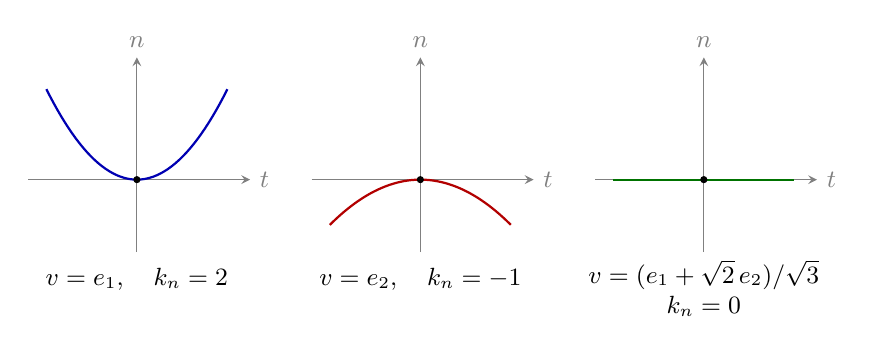
\begin{tikzpicture}[x=1.15cm,y=1.15cm,>=stealth,font=\small]
		\begin{scope}
			\draw[->,gray] (-1.2,0)--(1.25,0) node[right]{\(t\)};
			\draw[->,gray] (0,-0.8)--(0,1.35) node[above]{\(n\)};
			\draw[thick,blue!70!black,domain=-1:1,samples=50] plot(\x,{\x*\x});
			\fill (0,0) circle(1.3pt);
			\node at (0,-1.1){\(v=e_1,\quad k_n=2\)};
		\end{scope}
		\begin{scope}[xshift=3.6cm]
			\draw[->,gray] (-1.2,0)--(1.25,0) node[right]{\(t\)};
			\draw[->,gray] (0,-0.8)--(0,1.35) node[above]{\(n\)};
			\draw[thick,red!70!black,domain=-1:1,samples=50] plot(\x,{-0.5*\x*\x});
			\fill (0,0) circle(1.3pt);
			\node at (0,-1.1){\(v=e_2,\quad k_n=-1\)};
		\end{scope}
		\begin{scope}[xshift=7.2cm]
			\draw[->,gray] (-1.2,0)--(1.25,0) node[right]{\(t\)};
			\draw[->,gray] (0,-0.8)--(0,1.35) node[above]{\(n\)};
			\draw[thick,green!45!black] (-1,0)--(1,0);
			\fill (0,0) circle(1.3pt);
			\node[align=center] at (0,-1.2){\(v=(e_1+\sqrt2\,e_2)/\sqrt3\)\\\(k_n=0\)};
		\end{scope}
	\end{tikzpicture}
	\caption[鞍面在不同方向的法截线]{图像 \(z=x^2-\tfrac12y^2\) 在原点的三条法截线，各自画在由 \(v,n\) 张成的截平面内。三图的横坐标均沿单位切方向 \(v\)，纵坐标沿选定法向 \(n\)；相应截线为 \(z=t^2\)、\(z=-t^2/2\) 与 \(z=0\)。}
	\label{g1:fig:normal-sections}
\end{figure}


\subsection{平均曲率、Gauss 曲率及脐点}
\label{g1:subsec:0802:03}

两个主曲率交换编号时，和与积都不改变。把它们用于刻画曲面，可以避免不断选择和排列主方向。和反映两个正交方向的平均弯曲，积则区分同向弯曲、反向弯曲与二阶退化。

\begin{definition}[平均曲率、Gauss 曲率与脐点]\label{g1:def:surface-curvatures}
	在带选定单位法向的光滑浸入曲面上，定义\term[pingjunqulv]{平均曲率}[mean curvature]与\term[Gaussqulv]{Gauss 曲率}[Gaussian curvature]为
	\[
		H\coloneqq\tfrac12\operatorname{tr}S=\tfrac12(k_1+k_2),\qquad K\coloneqq\det S=k_1k_2.
	\]
	若某点 \(k_1=k_2\)，则称为\term[qidian]{脐点}[umbilic point]，等价地，该点 \(S=HI\)。若 \(S=0\)，称其为\term[pingdian]{平点}[planar point]；平点是两个主曲率都为零的脐点。
	\symidx{\(H\)：平均曲率}
	\symidx{\(K\)：曲面的 Gauss 曲率}
\end{definition}

这里的 \(1/2\) 属于平均曲率的约定，有些文献把主曲率之和直接叫作平均曲率。我们后续的公式均使用上面的平均值。Gauss 曲率目前是通过曲面在三维空间中的法向变化定义的；它是否也能仅由第一基本形式恢复，是下一节要证明的问题。

\begin{proposition}[曲率的计算与法向选择]\label{g1:prop:surface-curvature-formulas}
	设 \(X:U\to\mathbb R^3\) 是光滑浸入，选定单位法向，并使用第一、第二基本形式的系数 \(E,F,G,h_{ij}\)。则
	\begin{equation}\label{g1:eq:surface-HK-formulas}
		K=\frac{h_{11}h_{22}-h_{12}^2}{D},\qquad
		H=\frac{Gh_{11}-2Fh_{12}+Eh_{22}}{2D},\qquad D=EG-F^2.
	\end{equation}
	有 \(H^2-K\ge0\)，两个主曲率是 \(H\pm\sqrt{H^2-K}\)，脐点恰由 \(H^2=K\) 刻画。把法向改为 \(-n\) 时，\(S,\mathrm{II},H\) 同时变号，两个主曲率各自变号，\(K\) 与主方向不变。
\end{proposition}
\begin{proof}
	由\eqref{g1:eq:shape-matrix}，
	\[
		[S]=\frac1D
		\begin{pmatrix}
			Gh_{11}-Fh_{12}&Gh_{12}-Fh_{22}\\
			Eh_{12}-Fh_{11}&Eh_{22}-Fh_{12}
		\end{pmatrix}.
	\]
	取行列式和迹即得\eqref{g1:eq:surface-HK-formulas}。又
	\[
		H^2-K=\tfrac14(k_1-k_2)^2,\qquad
		\det(\lambda I-S)=\lambda^2-2H\lambda+K,
	\]
	所以平方根为实数，二次方程的根给出主曲率，等根恰为脐点。法向翻转后 \(S=-\mathrm dn\) 变号，其余各项由定义得到；若主曲率原先按大小排序，翻转后还须交换顺序。
\end{proof}

例如，外向法向的半径 \(R\) 球面处处有 \(H=-1/R\)、\(K=1/R^2\)，且每一点都是脐点。平面取任一固定单位法向则有 \(S=0\)。与此不同，图像 \(z=x^3-3xy^2\) 只在原点有二阶偏导全部为零，所以原点是平点；在其余位置，二阶偏导矩阵的行列式为 \(-36(x^2+y^2)\)，由图像公式及\eqref{g1:eq:surface-HK-formulas}知 \(K<0\)。因此“一点的第二基本形式为零”不意味着附近的曲面是一张平面。

\ProseParagraphBreak

平均曲率还真的是各方向法曲率的角平均。由 Euler 公式，
\[
	\frac1{2\pi}\int_0^{2\pi}k_n(\cos\theta\,e_1+\sin\theta\,e_2)\,\mathrm d\theta
	=\frac{k_1+k_2}2=H.
\]
平均值为零时，各方向的弯曲可能恰好抵消，不能据此断言每个方向都不弯曲。例如上一小节的鞍面若改为 \(z=x^2-y^2\)，则原点 \(H=0\) 而 \(K=-4\)。

\subsection{曲率线、渐近线及其退化}
\label{g1:subsec:0802:04}

一点上的方向能否沿曲面连成曲线，是另一个问题。先规定要沿哪些方向行走，再讨论方向能否光滑选取以及微分方程是否有解；这两步在脐点或曲率变号处都可能发生变化。

\begin{definition}[曲率线与渐近线]\label{g1:def:principal-asymptotic-curves}
	在带选定单位法向的光滑浸入曲面上，若一条光滑正则曲线的切向量处处为形算子的特征向量，称其为\term[qulvxian]{曲率线}[line of curvature]。若非零切向量 \(v\) 满足 \(\mathrm{II}(v,v)=0\)，称它张成的无向直线为\term[jianjinfangxiang]{渐近方向}[asymptotic direction]；切向量处处为渐近方向的光滑正则曲线称为\term[jianjinxian]{渐近线}[asymptotic curve]。
\end{definition}

法向翻转不改变特征方向，也不改变 \(\mathrm{II}(v,v)=0\) 的解，因此这两类曲线可以不依赖整体法向选择来讨论。曲率线要求法向变化 \(\mathrm dn(v)\) 与行进方向平行；渐近线要求曲线的法向加速度为零。两者是不同条件。

\begin{lemma}[局部积分曲线]\label{g1:lem:surface-field-integral-curve}
	设 \(V:U\to\mathbb R^2\) 是开集 \(U\subset\mathbb R^2\) 上的光滑向量场，\(u_0\in U\)。则在某个 \((-\varepsilon,\varepsilon)\) 上，初值问题
	\[
		\dot u(t)=V(u(t)),\qquad u(0)=u_0
	\]
	有唯一的局部光滑解。若 \(V(u_0)\ne0\)，缩小区间后该解正则。
\end{lemma}
\begin{proof}
	取闭球 \(\overline B(u_0,r)\subset U\)。由于 \(V\) 及其一阶导数在闭球上有界，存在常数 \(M,L\ge0\)，使 \(\lVert V\rVert\le M\) 且 \(\lVert V(x)-V(y)\rVert\le L\lVert x-y\rVert\)。选 \(a>0\) 足够小，使 \(aM<r\)、\(q=aL<1\)。在所有取值于此闭球的连续路径 \(u:[-a,a]\to\overline B(u_0,r)\) 上定义
	\[
		(\mathcal Tu)(t)=u_0+\int_0^t V(u(s))\,\mathrm ds.
	\]
	估计 \(aM<r\) 保证 \(\mathcal T\) 仍取值于闭球，而一致范数满足
	\[
		\lVert\mathcal Tu-\mathcal Tw\rVert_\infty\le q\lVert u-w\rVert_\infty.
	\]
	从常路径 \(u_0\) 迭代 \(u_{m+1}=\mathcal Tu_m\)，相邻两次的差至多按 \(q^m\) 衰减。几何级数收敛说明 \(u_m\) 一致收敛；连续路径的一致极限仍连续且取值于闭球。把极限送入积分，得到 \(u=\mathcal Tu\)，所以 \(u\) 为 \(C^1\) 且满足方程。若 \(u,w\) 都是这个积分方程的解，同一估计给出 \(\lVert u-w\rVert_\infty\le q\lVert u-w\rVert_\infty\)，因而两者相同。任意另一局部解在足够短的公共区间内也留在闭球中，这就给出局部唯一性。由 \(\dot u=V(u)\) 逐次求导，\(u\) 为光滑；最后用 \(V(u_0)\ne0\) 及连续性保证附近速度不消失。
\end{proof}

\begin{proposition}[主方向与渐近方向的局部曲线]\label{g1:prop:principal-asymptotic-lines}
	设 \(X:U\to\mathbb R^3\) 为光滑浸入。
	\begin{enumerate}
		\item 每个非脐点附近有两族局部曲率线；经过给定点、沿指定主方向的局部曲率线唯一到正则重参数化为止。
		\item 每个 \(K<0\) 的点附近有两族局部渐近线；经过给定点、沿指定渐近方向的局部渐近线唯一到正则重参数化为止。
		\item 在一点，若 \(K>0\)，没有渐近方向；若 \(K<0\)，有两条不同的渐近方向；若 \(K=0\) 且 \(S\ne0\)，恰有一条渐近方向，为 \(\ker S\)；若 \(S=0\)，所有方向都是渐近方向。
	\end{enumerate}
\end{proposition}
\begin{proof}
	在非脐点附近，\(H^2-K>0\)。所以
	\[
		k_+=H+\sqrt{H^2-K},\qquad k_-=H-\sqrt{H^2-K}
	\]
	是光滑的不同特征值。相应的线性算子
	\[
		P_+=\frac{S-k_-I}{k_+-k_-},\qquad P_-=\frac{S-k_+I}{k_--k_+}
	\]
	分别投影到两条特征直线上。先取一个光滑切向量场 \(W\)，使 \(P_+W\) 在指定点不为零；例如把该点的一个特征向量按坐标基用常系数延伸。缩小邻域后 \(P_+W\) 始终不为零，归一化得到光滑单位特征向量场 \(e_+\)。同理得到 \(e_-\)，并可按需要调整其符号。把 \(e_+\) 在 \(X_1,X_2\) 下的系数看作 \(U\) 上的非零光滑向量场，应用\cref{g1:lem:surface-field-integral-curve}并复合 \(X\)，即得所需曲率线。另一主方向同样处理。任意沿同一方向的正则曲线，缩短后可调整方向并改用弧长，使其导数等于所选单位场；初值唯一性就给出无参数轨迹的唯一性。

	当 \(K<0\) 时，\(k_+>0>k_-\)。在上面选出的光滑正交单位场中，二次型的零方向由
	\[
		k_+a^2+k_-b^2=0
	\]
	确定，分别由两个光滑非零场
	\[
		\sqrt{-k_-}\,e_++\sqrt{k_+}\,e_-,
		\qquad
		\sqrt{-k_-}\,e_+-\sqrt{k_+}\,e_-
	\]
	张成。归一化后再次应用局部积分曲线引理，得到存在与唯一性。

	最后，在任一点用主方向正交基把 \(\mathrm{II}\) 写成 \(k_1a^2+k_2b^2\)。若两系数同号，此式对非零向量不为零；若异号，得到上面的两条直线；若恰有一个系数为零，解是一条坐标轴；若两者都为零，每个向量都是解。这证明了第三项。
\end{proof}

这份分类只需解一个二元二次方程，可整理为\cref{g1:tab:asymptotic-directions}。其中 \(K=0\) 的两行必须分开：仅凭 \(K\) 的值，无法判断零方向是一条还是所有方向。

\begin{table}[htbp]
	\centering
	\caption{第二基本形式与渐近方向}
	\label{g1:tab:asymptotic-directions}
	\begin{tabular}{lll}
		\toprule
		条件 & 主方向基下的二次型 & 渐近方向 \\
		\midrule
		\(K>0\) & 两个非零系数同号 & 无 \\
		\(K<0\) & 两个系数异号 & 两条不同直线 \\
		\(K=0,\ S\ne0\) & 恰有一个系数为零 & 一条直线 \\
		\(S=0\) & 零二次型 & 所有方向 \\
		\bottomrule
	\end{tabular}
\end{table}

在一整片 \(K=0,\ S\ne0\) 的区域上，零特征值与另一个特征值仍然分离，上面的投影构造同样给出一条光滑方向场及其积分曲线。但若只知道某一点 \(K=0\)，不能据此断言有渐近线穿过它。例如 \(z=x^2+y^4\) 在原点的形算子为 \(\operatorname{diag}(2,0)\)，只有 \(y\) 轴方向渐近；在 \(y\ne0\) 处却有 \(K>0\)，不存在渐近方向。若有正则渐近线通过原点，其速度必须沿 \(y\) 轴且不为零，于是附近离开原点后 \(y\ne0\)，矛盾。因此原点的渐近方向不能延续成穿过该点的渐近线。

\ProseParagraphBreak

脐点处的困难则是主方向不再分离。球面的每条正则曲线都是曲率线，经过一点和一条切向的曲线远不唯一。即使避开脐点，在一张较大的曲面上也不能从局部单位特征向量的选择自动得到全局连续选择：沿闭路延伸后，向量可能反向，而它张成的直线仍相同。曲率线和渐近线的定义使用无向直线，正是为了把这种方向选择与曲线本身区别开。
